\documentclass[11pt]{article}

\usepackage{acl2013}
\usepackage{times}
\usepackage{latexsym}
\usepackage{amsmath}
\usepackage{multirow}
\usepackage{array}
\usepackage{url}
\usepackage{graphicx}
\usepackage{subfig}
\usepackage{marvosym}
\usepackage{todonotes}

\setlength\titlebox{6.5cm}

\newcommand{\mnote}[1]{\marginpar{%
  \vskip-\baselineskip
  \raggedright\footnotesize
  \itshape\hrule\smallskip\footnotesize{#1}\par\smallskip\hrule}}

%% \newcommand{\aff}{\ensuremath{{}^\text{\Radioactivity}}}
%% \newcommand{\afff}{\ensuremath{{}^\text{\Bat}}}
\newcommand{\hltcoe}{\ensuremath{{}^\text{1}}}
\newcommand{\clsp}{\ensuremath{{}^\text{2}}}
\newcommand{\upenn}{\ensuremath{{}^\text{2}}}
\newcommand{\grammarrule}[3]{$#1 \to \langle \text{#2} , \text{#3} \rangle$ }

\title{Joshua 5.0: Sparse features, performance enhancements, and improved grammar extraction}

\author{Matt Post\hltcoe 
  \and Juri Ganitkevitch\clsp 
  \and Luke Orland\hltcoe
  \and Jonathan Weese\clsp
  \and Yuan Cao\clsp  \\
  \clsp Center for Language and Speech Processing \\
  \hltcoe Human Language Technology Center of Excellence \\
  Johns Hopkins University \\
  \AND  Chris Callison-Burch \\
  Computer and Information Sciences Department \\
  University of Pennsylvania \\
}

\date{}

\begin{document}
\maketitle

\begin{abstract}
  We describe improvements made over the past year to Joshua, an
  open-source translation system for parsing-based translation. The
  main contributions this past year are significant improvements in
  both speed and usability of the grammar extraction and decoding
  steps. We have also rewritten the decoder to use a sparse feature
  representation, enabling training of large numbers of features with
  discriminative training methods.
\end{abstract}

%%%%%%%%%%%%%%%%%%%%%%%%%%%%%%%%%%%%%%%%%%%%%%%%%%%%%%%%%%%%%%%%%
\section{Introduction}
\label{sec-intro}

Joshua is an open-source toolkit\footnote{\url{joshua-decoder.org}}
for hierarchical and syntax-based statistical machine translation of
human languages.  The original version of Joshua \cite{Joshua-WMT} was
a port (from Python to Java) of the Hiero machine translation system
introduced by \newcite{Chiang2007}.  It was later extended to support
grammars with rich syntactic labels \cite{li2010joshua}. Subsequent
efforts produced Thrax, the extensible Hadoop-based extraction tool
for synchronous context-free grammars \cite{Joshua-3.0}, which was
later extended to support pivoting-based paraphrase extraction
\cite{Joshua-4.0}. Joshua 5.0 continues our yearly update cycle and is
the fourth formal release.

Here are a summary of the major components of Joshua 5.0:

\begin{itemize}
  \item[\S\ref{sec:sparse}] \emph{Sparse features}. Joshua now supports an
    easily-extensible sparse feature implementation, along with tuning
    methods (PRO and kbMIRA) for efficiently setting the weights on
    large feature vectors.
  \item[\S\ref{sec:performance}] \emph{Significant speed
    increases}. Joshua 5.0 is up to six times faster than Joshua 4.0,
    and also does well against hierarchical Moses, where end-to-end
    decoding (including model loading) of WMT test sets is as much as
    three times faster (although, in the limit, sentence-level
    throughput is only half that of Moses)
  \item[\S\ref{sec:thrax}] \emph{Thrax 2.0}. A reengineered Thrax is
    up to 300\% faster while using significantly less intermediate
    disk space.
  \item[\S\ref{sec:other}] \emph{Many other features}. This release
    contains a number of other features, including a server mode with
    fair round-robin scheduling among and within requests, a bundler
    for easily packaging up a trained model, improvements to the
    Joshua pipeline (for managing end-to-end experiment), and better
    end-user documentation.
\end{itemize}

%%%%%%%%%%%%%%%%%%%%%%%%%%%%%%%%%%%%%%%%%%%%%%%%%%%%%%%%%%%%%%%%%
\section{Overview}

Joshua is an open-source end-to-end statistical machine translation
toolkit. In addition to the decoder component (which performs the
actual translation), it includes the support infrastructure needed to
prepare and align training data, build translation and language
models, tune a system, and evaluate it against test data. 

This section provides a brief overview of the contents and abilities
of this toolkit.

\subsection{The Pipeline: Gluing it all together}

The Joshua pipeline ties together all the infrastructure needed to
train and evaluate machine translation systems for research or
industrial purposes. Once data has been segmented into parallel
training, development, and test sets, a single invocation of the
pipeline script is enough to invoke this entire infrastructure from
beginning to end. Each step is broken down into smaller steps (e.g.,
tokenizing a file) whose results are cached using SHA-1 sums. This
allows a reinvoked pipeline to easily skip earlier steps that do not
need to be recomputed, solving a common headache in the research and
development cycle.

The Joshua pipeline is similar to other ``experiment
management systems'' such as that included with Moses.  Moses'
\verb|Experiment.perl| is a much more general, highly-customizable
tool that allows the specification and parallel execution of
customizable steps in arbitrary dependency graphs, much like the
\textsc{Unix} \verb|make| tool, but written with machine translation
in mind. Joshua's pipeline is much more limited in that the pipeline
is hard-coded. However, this reduced versatility covers many standard
use cases and is arguably easier to use. 

The pipeline is parameterized in many ways, and all the options below
are selectable with command-line switches. Pipeline documentation is
available online.

\subsection{Data preparation, Alignment, and Model building}

Data preparation involves data normalization (e.g., collapsing certain
punctuation symbols) and tokenization (via the Penn treebank
tokenizer).  Alignment with GIZA++ \cite{giza} and the Berkeley aligner
\cite{berkeley-aligner} are supported.

Joshua's builtin grammar extractor, Thrax, is a Hadoop-based
extraction implementation that scales easily to large datasets. It
supports extraction of both Hiero \cite{Chiang2005} and SAMT grammars
\cite{samt2006} with extraction heuristics easily specified via a
flexible configuration file. The pipeline also supports GHKM grammar
extraction \cite{galley2006scalable} using the extractors available
from Michel
Galley\footnote{\url{nlp.stanford.edu/~mgalley/software/stanford-ghkm-latest.tar.gz}}
or Moses.

SAMT and GHKM grammar extraction requires a parse tree, which are
produced over the training data using the Berkeley parser \cite{petrov2006learning}.

\subsection{Decoding}

The Joshua decoder is an implementation of the CKY+ algorithm
\cite{chappelier1998generalized}, which generalizes CKY by removing
the requirement that the grammar first be converted to Chomsky Normal
Form, thereby avoiding the complexities of many binarization schemes
\cite{zhang2006synchronous,denero2009asynchronous}. CKY+ maintains
cubic-time parsing complexity (in the sentence length) with
Earley-style implicit binarization of rules. Joshua works natively
with arbitrary synchronous context-free grammars (SCFGs), imposing no
limitation on the rank or form of grammar rules. 

Parsing complexity is still exponential in the rank of the grammar, so
grammar filtering remains important.  The default Thrax settings
extract only grammars with rank 2, and the pipeline implements scope-3
pruning \cite{hopkins2010scfg} when filtering grammars to test sets
(for GHKM). 

Joshua uses cube pruning \cite{Chiang2007} with a default pop limit of
100 to efficiently explore the search space.

\subsection{Tuning and Testing}

Joshua ships with MERT \cite{Och2003} and PRO implementations.  Tuning
with k-best batch MIRA \cite{cherry2012batch} is also supported, but requires
Moses to be installed.


%%%%%%%%%%%%%%%%%%%%%%%%%%%%%%%%%%%%%%%%%%%%%%%%%%%%%%%%%%%%%%%%%
\section{What's New in Joshua 5.0}

\subsection{Sparse features}
\label{sec:sparse}

Until a few years ago, machine translation systems were for the most
part limited in the number of features they could employ, since the
line-based optimization method, MERT \cite{Och2003}, was not able to
efficiently search over more than tens of feature weights.  The
introduction of discriminative tuning methods for machine translation
\cite{liang2006end,tillmann-zhang:2006:COLACL,chiang2008online,PRO2011}
has made it possible to tune large numbers of features in statistical
machine translation systems, and open-source implementations such as
\newcite{cherry2012batch} have made it easy.  When dealing with large
numbers of features (on the order of thousands), it is important that
they be represented in a sparse format, particularly since large
feature sets often employ many binary-valued features, a large number
of which are zero for any particular edge in the hypergraph.

Joshua 5.0 has moved to a sparse feature representation
internally. First, to clarify terminology, a feature as implemented in
the decoder is actually a template that can introduce any number of
actual features (in the standard machine learning sense). We will use
the term \emph{feature function} for these templates and
\emph{feature} for the individual, traditional features that are
induced by these templates. For example, the (typically dense)
features stored with the grammar on disk are each separate features
contributed by the \textsc{PhraseModel} feature function template. The
\textsc{LanguageModel} template contributes a single feature value for
each language model that was loaded (typically one).

For performance reasons, during decoding, Joshua does not maintain the
entire feature vector associated with nodes in the forest hypergraph.
Instead, nodes maintain only the best cumulative score of each
incoming hyperedge, and the edges themselves retain only the hyperedge
delta (the inner product of the weight vector and features incurred by
that edge).  After decoding, the entire feature vector can be
recomputed if that information is required by the caller of the
decoder.  

This functionality is implemented via the following
feature function interface (simplified pseudocode):
%
\begin{verbatim}
  interface FeatureFunction:
    apply(context, accumulator)
\end{verbatim}
%
The \verb|context| comprises fixed pieces of the input sentence and
hypergraph:
%
\begin{itemize}
\item the hypergraph edge (which represents the SCFG rule and sequence
  of tail nodes)
\item the complete source sentence
\item the input span
\end{itemize}
%
The \verb|accumulator| object's job is to accumulate feature
(name,value) pairs by a feature function during the application of a
rule via another interface:
%
\begin{verbatim}
  interface Accumulator:
    add(feature_name, value)
\end{verbatim}
%
The accumulator generalization,\footnote{Due to Kenneth Heafield.}
allows us use a single feature-gathering function for two accumulator
objects: one, used during decoding, maintains and eventually returns
only a weighted sum, and the second, used (if needed) during k-best
extraction, constructs a sparse feature vector.

For tuning large sets of features, Joshua supports both PRO
\cite{PRO2011}, an in-house version introduced with Joshua 4.0, and
k-best batch MIRA \cite{cherry2012batch}, implemented via integration
with code available in Moses.

\subsection{Performance improvements}
\label{sec:performance}

We introduced many performance improvements, replacing code designed
to get the job done under research timeline constraints with more
efficient alternatives, including smarter handling of locking among
threads, more efficient (non string-based) computation of dynamic
programming state, and replacement of fixed class-based array
structures with fixed-size literals.

We used the following experimental setup to compare Joshua 4.0 and
5.0: We extracted a large German-English grammar from all sentences
with no more than 50 words per side from Europarl v.7
\cite{koehn2005europarl} and the Common Crawl data using Thrax default
settings.  After filtering against our test set (newstest2012), this
grammar contained 70 million rules.  We then trained three language
models on (1) the target side of our grammar training data, (2)
English Gigaword, and (3) the monolingual English data released for
WMT13. We tuned a system using kbMIRA and decoded using KenLM
\cite{KenLM}.  Decoding was performed on 64-core 2.1 GHz AMD Opteron
processors with 256 GB of available memory.

Figure~\ref{fig:cmp} plots the end-to-end runtime\footnote{i.e.,
  including model loading time and grammar sorting.} as a function of
the number of threads.  Each point in the graph is the minimum of at
least fifteen runs computed at different times over a period of a few
days.  The main point of comparison, between Joshua 4.0 and 5.0, shows
that the current version is up to 500\% faster than it was last year,
especially in multithreaded situations.

\begin{figure}[!t]
  \begin{center}
    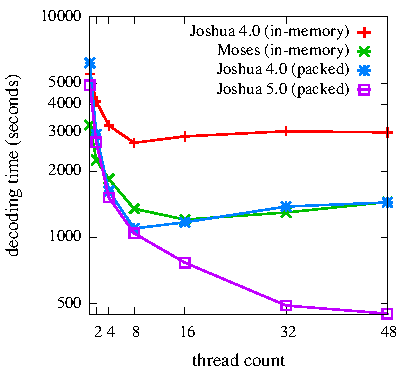
\includegraphics[width=0.99\linewidth]{plots/runtimes.pdf}
  \end{center}
  \caption{End-to-end runtime as a function of the number of threads
    for Joshua 4.0, Joshua 5.0, and Moses. Each data point is the
    minimum of at least fifteen different runs taken at different
    times over multiple days.}
  \label{fig:cmp}
\end{figure}

\begin{figure}[!t]
  \begin{center}
    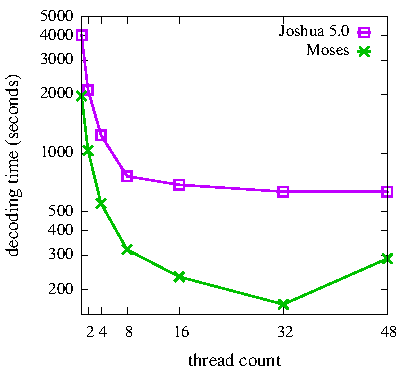
\includegraphics[width=0.99\linewidth]{plots/decoding-only.pdf}
  \end{center}
  \caption{Decoding time alone, having subtracted out model loading
    and sorting times as reported in log files.}
  \label{fig:decoding-only}
\end{figure}

For further comparison, we took these models, converted them to
hierarchical Moses format, and then decoded with the latest
version.\footnote{The latest version available on Github as of June 7,
  2013} We compiled Moses with the all the recommended optimization
settings \footnote{With tcmalloc and the following compile flags:
  \texttt{--max-factors=1 --kenlm-max-order=5 debug-symbols=off}} and
used the in-memory (SCFG) grammar format.  BLEU scores were
similar.\footnote{22.88 for Moses, 22.99 for Joshua 4.0, and 23.23 for
  Joshua 5.0.}  Figure~\ref{fig:cmp} shows that, in this end-to-end
setting, Joshua is about 200\% faster than Moses at high thread
counts.

Figure \ref{fig:decoding-only} furthers the comparison between Joshua
and Moses by plotting only decoding time (that is, subtracting out
model loading and sorting times). Moses' decoding speed is about twice
that of Joshua, which shows that the end-to-end gains in
Figure~\ref{fig:cmp} are due to more efficient grammar loading.

\subsection{Thrax 2.0}
\label{sec:thrax}

The Thrax module of our toolkit has undergone a similar overhaul. The
rule extraction code was rewritten to be easier to understand and
extend, allowing, for instance, for an easy inclusion of alternative
nonterminal labeling strategies.

\begin{table*}[t]
  \begin{center}
    \begin{tabular}{|c|r|r|r|r|r|r|r|r|}
      \hline
      & \multicolumn{2}{c|}{Cs-En} & \multicolumn{2}{c|}{Fr-En} &
      \multicolumn{2}{c|}{De-En} & \multicolumn{2}{c|}{Es-En} \\

      Rules & \multicolumn{2}{c|}{112M} & \multicolumn{2}{c|}{357M} &
      \multicolumn{2}{c|}{202M} & \multicolumn{2}{c|}{380M} \\

      \hline

      & \multicolumn{1}{c|}{Space} & \multicolumn{1}{c|}{Time} &
      \multicolumn{1}{c|}{Space} & \multicolumn{1}{c|}{Time}  &
      \multicolumn{1}{c|}{Space} & \multicolumn{1}{c|}{Time}  &
      \multicolumn{1}{c|}{Space} &  \multicolumn{1}{c|}{Time} \\
      \hline
      \hline
      Joshua 4.0 & 120GB & 112 min & 364GB & 369 min & 211GB & 203 min & 413GB & 397 min \\
      \hline
      Joshua 5.0 & 31GB  & 25 min & 101GB  & 81 min & 56GB  & 44 min & 108GB & 84 min \\
      \hline
      \hline
      Difference & -74.1\% & -77.7\%  & -72.3\% & -78.0\%  & -73.5\% & -78.3\%  & -73.8\% & -78.8\% \\
      \hline
    \end{tabular}
  \end{center}
  \caption{Comparing Hadoop's intermediate disk space use and
    extraction time on a selection of Europarl v.7 Hiero grammar
    extractions. Disk space was measured at its maximum, at
    the input of Thrax's final grammar aggregation stage. Runtime was
    measured on our Hadoop cluster with a capacity of 52 mappers and
    26 reducers. On average Thrax 2.0, bundled with Joshua 5.0,
    is up to 300\% faster and more compact.}
  \label{tab-thrax-speed}
\end{table*}

We optimized the data representation used for the underlying
map-reduce framework towards greater compactness and speed --
resulting in a 300\% increase in extraction speed and an equivalent
reduction is disk I/O (see Table~\ref{tab-thrax-speed}). These gains
enable us to extract a syntactically labeled De-En SAMT-style
translation grammar from a bitext of over 4 million sentence pairs in
just over 3 hours. Furthermore, Thrax 2.0 is capable of scaling to
very large data sets, like the composite bitext used in the extraction
of the paraphrase collection PPDB \cite{PPDB}, which counted 100
million sentence pairs and over 2 billion words on the English side.

\begin{figure}
  \centering
  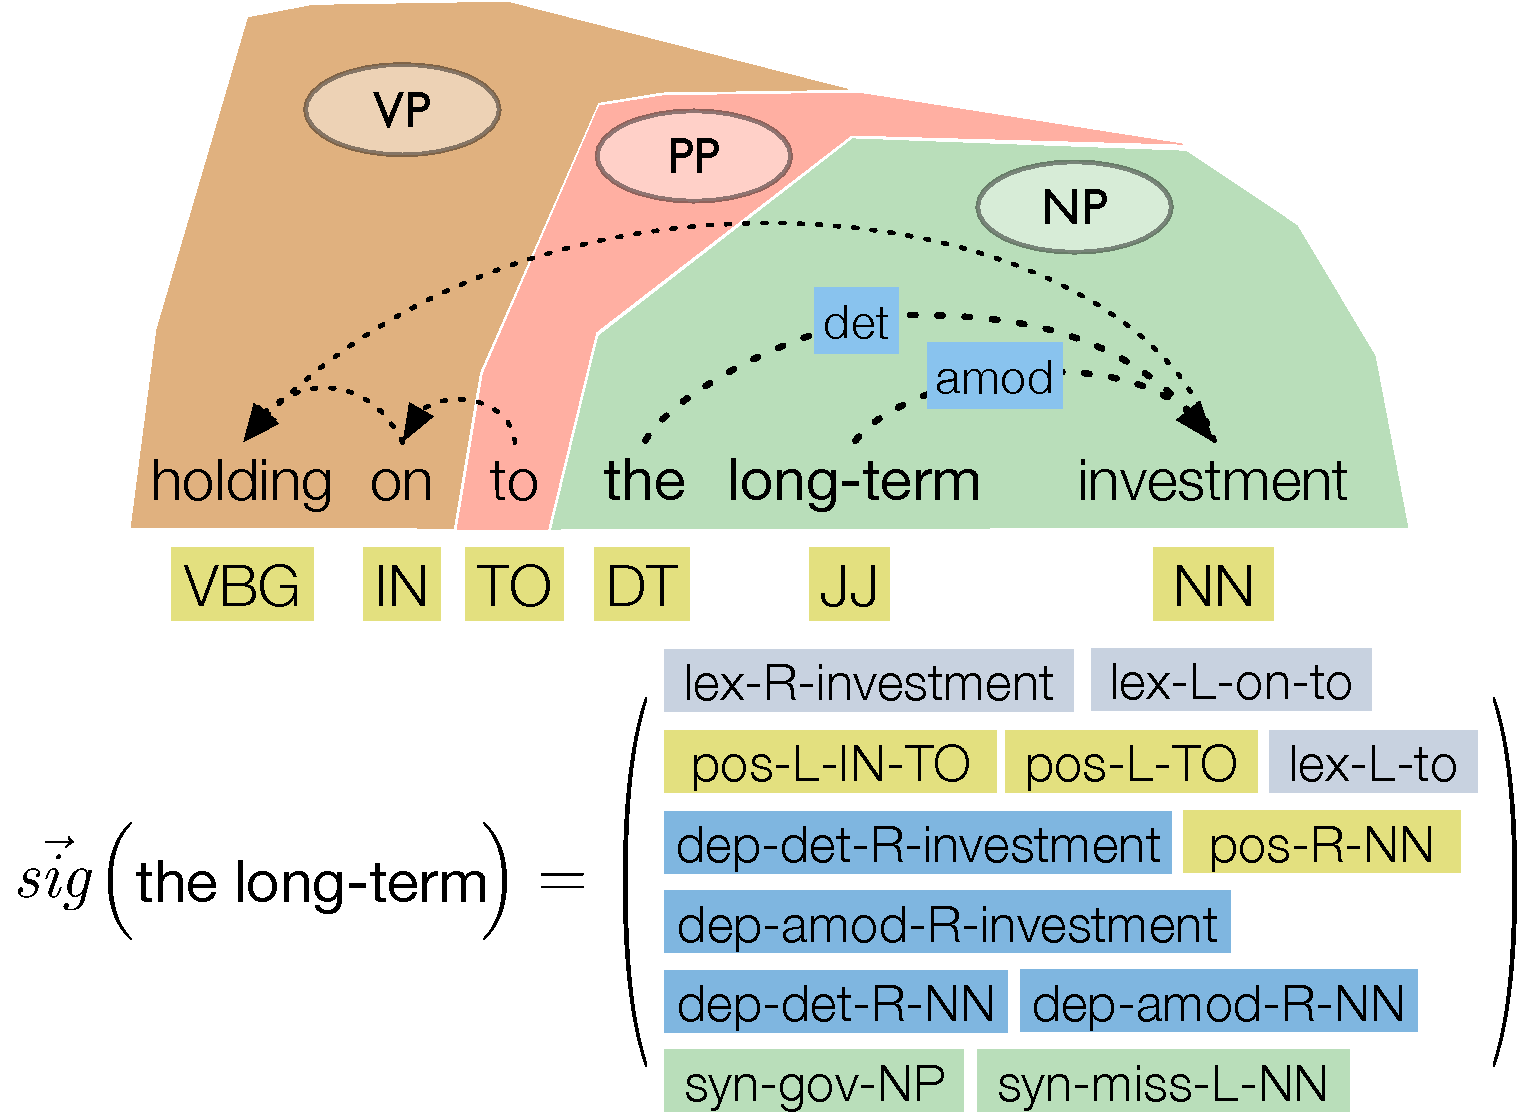
\includegraphics[ width=0.95\linewidth]{figures/rich_context.pdf}
  \caption{\small Here, position-aware lexical and part-of-speech
    $n$-gram features, labeled dependency links , and features
    reflecting the phrase's CCG-style label $\mathit{NP/NN}$ are
    included in the context vector.}\label{fig-rich-context}
\end{figure}

Furthermore, Thrax 2.0 contains a module focused on the extraction of
compact distributional signatures over large datasets. This
\emph{distributional} mode collects contextual features for $n$-gram
phrases, such as words occurring in a window around the phrase, as
well as dependency-based and syntactic
features. Figure~\ref{fig-rich-context} illustrates the feature
space. We then compute a bit signature from the resulting feature
vector via a randomized locality-sensitive hashing projection.  This
yields a compact representation of a phrase's typical context. To
perform this projection Thrax relies on the Jerboa toolkit
\cite{Jerboa}. As part of the PPDB effort, Thrax has been used to
extract rich distributional signatures for 175 million 1-to-4-gram
phrases from the Annotated Gigaword corpus \cite{annotated-gigaword},
a parsed and processed version of the English Gigaword
\cite{Gigaword}.

\subsection{Other features}
\label{sec:other}

Joshua 5.0 also includes many features designed to increase its
usability as a research and application tool.  These include:

\begin{itemize}
\item A TCP/IP server architecture for networked installations.  This
  setup interactions with Joshua's internal multithreading
  implementation, which is designed to handle multiple sets of
  translation requests, ensuring fairness in thread assignment both
  across and within these connections.
\item A bundler that makes it easy to package up a trained model with
  all of its support files and dependencies.
\item A year's worth of improvements to the Joshua pipeline, including many
  new features and supported options, and increased robustness to error.
\item Extended end-user and developer documentation.
\end{itemize}

%%%%%%%%%%%%%%%%%%%%%%%%%%%%%%%%%%%%%%%%%%%%%%%%%%%%%%%%%%%%%%%%%
\section{Summary}

The 5.0 release of Joshua is the result of a significant year-long
research, engineering, and usability effort that we hope will be of
service to the research community. 

\paragraph{Acknowledgements}

Joshua's sparse feature representation owes much to discussions with
Colin Cherry, Barry Haddow, Chris Dyer, and Kenneth Heafield at MT
Marathon 2012 in Edinburgh.

This material is based on research sponsored by the NSF under grant
IIS-1249516 and DARPA under agreement number FA8750-13-2-0017 (the
DEFT program).  The U.S.\ Government is authorized to reproduce and
distribute reprints for Governmental purposes.  The views and
conclusions contained in this publication are those of the authors and
should not be interpreted as representing official policies or
endorsements of DARPA or the U.S. Government.


%% This research was supported by in part by the EuroMatrixPlus project
%% funded by the European Commission (7th Framework Programme), and by
%% the NSF under grant IIS-0713448. Opinions, interpretations, and
%% conclusions are the authors' alone.

\bibliographystyle{acl2013}
\bibliography{joshua}

\end{document}
